% ==================================================================
%  Section 2.7 – Layer Fusion
% ==================================================================
\section{Layer Fusion}
\label{sec:bg-layer-fusion}

All preceding sections have implicitly assumed that only a
\emph{single} convolution (or GEMM) is mapped at a time: the
accelerator reads one layer's inputs and weights from DRAM, computes
its outputs, writes them back to DRAM, and then moves on to the next
layer.
Under this \textbf{layer-by-layer} (LBL) execution model, every
intermediate feature map must traverse the full memory hierarchy twice—once
as the output of one layer and once as the input to the next.
Since DRAM accesses dominate the energy budget
(Section~\ref{sec:energy-model}), these redundant round-trips constitute a
major source of inefficiency in modern DNN inference.

\textbf{Layer fusion} is the strategy of co-executing two or more
consecutive layers so that intermediate feature maps are produced
\emph{and consumed on-chip}, without ever being written to DRAM.
This section introduces the concept, formalizes its mechanics, and
discusses the open problems it raises.

% ------------------------------------------------------------------
\subsection{Motivation}
\label{sec:fusion-motivation}

Consider a network of $N$ consecutive layers
$\mathcal{L}_0, \mathcal{L}_1, \dots, \mathcal{L}_{N-1}$, executed layer by
layer.  Let $A_i$ denote the intermediate activation tensor between
$\mathcal{L}_i$ and $\mathcal{L}_{i+1}$.
In LBL execution, each $A_i$ is written to DRAM after
$\mathcal{L}_i$ completes and read back when $\mathcal{L}_{i+1}$
starts, incurring
\begin{equation}
\label{eq:lbl-traffic}
T_{\text{LBL}}^{\text{intermediate}}
  \;=\; 2\,\sum_{i=0}^{N-2} |A_i|
\end{equation}
DRAM accesses (one write plus one read per element).  For deep networks with
large spatial resolutions, this traffic can far exceed the traffic for inputs,
outputs, and weights combined.  For instance, in the early layers of
VGG-16~\cite{simonyan2015very}, the intermediate feature maps of a single
$224\!\times\!224$ image occupy tens of megabytes—orders of magnitude
larger than the corresponding filter weights.

When $F$ consecutive layers ($\mathcal{L}_0$ through
$\mathcal{L}_{F-1}$) are \emph{fused}, all $F-1$ intermediate tensors
$A_0, \dots, A_{F-2}$ are kept on-chip and ideally never touch DRAM.
The DRAM traffic for the fused group therefore reduces to
\begin{equation}
\label{eq:fused-traffic}
T_{\text{fused}}
  \;=\; \underbrace{|I|}_{\text{first layer's input}}
  \;+\; \underbrace{\sum_{i=0}^{F-1}|W_i|}_{\text{all weights}}
  \;+\; \underbrace{|O|}_{\text{last layer's output}},
\end{equation}
eliminating the intermediate traffic entirely.

% ------------------------------------------------------------------
\subsection{Fused Tiling}
\label{sec:fused-tiling}

Fusion does not simply mean running all layers in sequence inside a
single invocation.
The key insight is that the tiling of the outer (last) layer's output
\emph{dictates} the tiles required from every preceding layer through
a chain of producer--consumer dependencies.

\begin{figure}[t]
\centering
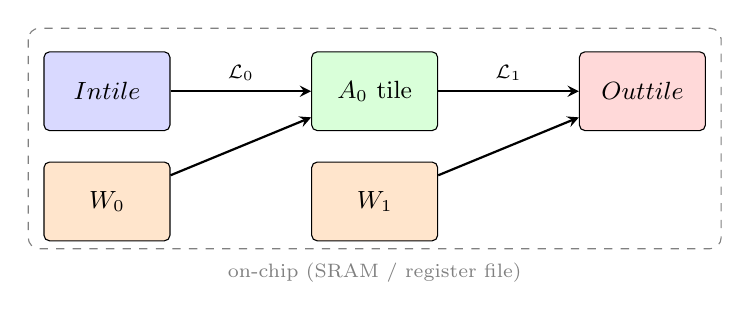
\begin{tikzpicture}[
    tile/.style={draw, minimum width=1.6cm, minimum height=1.0cm,
                 rounded corners=2pt, font=\small},
    arr/.style={->, >=stealth, thick}
  ]
  % Layer 0
  \node[tile, fill=blue!15] (in) at (0,0) {$\text{In tile}$};
  \node[tile, fill=orange!20] (w0) at (0,-1.4) {$W_0$};
  % Layer 0 output = intermediate
  \node[tile, fill=green!15] (a0) at (3.4,0) {$A_0$ tile};
  % Layer 1
  \node[tile, fill=orange!20] (w1) at (3.4,-1.4) {$W_1$};
  % Layer 1 output
  \node[tile, fill=red!15] (out) at (6.8,0) {$\text{Out tile}$};

  \draw[arr] (in) -- node[above, font=\scriptsize]{$\mathcal{L}_0$} (a0);
  \draw[arr] (w0) -- (a0);
  \draw[arr] (a0) -- node[above, font=\scriptsize]{$\mathcal{L}_1$} (out);
  \draw[arr] (w1) -- (out);

  % On-chip annotation
  \draw[dashed, gray, rounded corners=4pt]
    (-1.0, 0.8) rectangle (7.8, -2.0);
  \node[gray, font=\scriptsize] at (3.4, -2.3) {on-chip (SRAM / register file)};
\end{tikzpicture}
\caption{Fused execution of two consecutive layers.  The intermediate
  activation~$A_0$ is produced and consumed on-chip; only the network's
  input, weights, and final output cross the DRAM boundary.}
\label{fig:fused-two-layers}
\end{figure}

Consider fusing two convolutional layers with filter sizes
$R_0\!\times\!S_0$ and $R_1\!\times\!S_1$ respectively.
If the second layer requires an output tile of size $P\!\times\!Q$, it
needs an intermediate tile of size
$(P+R_1-1)\times(Q+S_1-1)$ from the first layer's output
(cf.\ the halo discussion in Section~\ref{sec:loop-ordering}).
To produce that intermediate tile, the first layer in turn needs an input
tile of size
\begin{equation}
\label{eq:fused-input-tile}
\bigl(P + R_1 - 1 + R_0 - 1\bigr) \times
\bigl(Q + S_1 - 1 + S_0 - 1\bigr).
\end{equation}
The tile sizes thus \emph{cascade backwards} through the fused layers,
and each intermediate tile is enlarged by its layer's corresponding
halo.  This cascading is precisely the phenomenon captured by
\emph{affine dimensions} (Definition~\ref{def:affine-dim} in
Section~\ref{sec:normal-affine}): the sums of indices (e.g.\ $p + r_1$
mapping to intermediate spatial positions) create dependencies that
propagate tile-size requirements across layers.

\paragraph{Memory-footprint implications.}
All intermediate tiles must fit simultaneously in an on-chip buffer,
since they are produced and consumed between consecutive loop
iterations without visiting DRAM.
Let $\text{FMEM}$ denote the on-chip feature memory.  In the two-layer
case the buffer must hold at least:
\begin{equation}
\label{eq:fused-footprint}
\text{footprint}
  \;\geq\;
  \underbrace{|I_{\text{tile}}|}_{\text{input tile}}
  +\;
  \underbrace{|A_{0,\text{tile}}|}_{\text{intermediate tile}}
  +\;
  \underbrace{|O_{\text{tile}}|}_{\text{output tile}}.
\end{equation}
As more layers are fused, additional intermediate tiles must be stored
concurrently, increasing the footprint.  Correspondingly, the output
tile size $P\!\times\!Q$ that fits within a given FMEM budget
\emph{decreases} with the number of fused layers, which can impact
data reuse and, in turn, energy efficiency.

% ------------------------------------------------------------------
\subsection{Multi-Layer Workload Formalization}
\label{sec:multi-layer-workload}

Section~\ref{sec:bg-workloads} formalized a single-layer computation as a
loop nest with a coupling that maps dimensions to operands.
Fusion extends this formalization: a fused group of $F$ layers is
expressed as a \emph{single, unified loop nest} whose coupling now defines
five categories of operands instead of three:
\begin{enumerate}
  \item \textbf{Input} (\texttt{in})—read-only tensor consumed by the
        first layer.
  \item \textbf{Weights} (\texttt{w})—one per layer ($W_0, \dots, W_{F-1}$),
        each referenced only by its own layer's dimensions.
  \item \textbf{Intermediate output} (\texttt{int\_out})—the output
        produced by every layer except the last; for layer~$i$ this is
        $A_i$.
  \item \textbf{Intermediate input} (\texttt{int\_in})—the input consumed
        by every layer except the first; layer~$i$ reads $A_{i-1}$, which
        is the \texttt{int\_out} of the previous layer.
  \item \textbf{Output} (\texttt{out})—write-only tensor produced by the
        last layer.
\end{enumerate}

In the Extended Einsum Notation (Section~\ref{sec:een}), a two-layer
fused convolution is written as:
\begin{align}
\label{eq:een-fused-2layer}
A_0[z_0, y_0, x_0] &\mathrel{+}= W_0[z_0, c_0, r_0, s_0]
  \cdot \text{In}[c_0, y_0\!+\!r_0, x_0\!+\!s_0], \notag\\[2pt]
\text{Out}[z_1, p, q] &\mathrel{+}= W_1[z_1, c_1, r_1, s_1]
  \cdot A_0[c_1, p\!+\!r_1, q\!+\!s_1].
\end{align}
All twelve dimensions ($C_0, Y_0, X_0, R_0, S_0, Z_0, C_1, R_1,
S_1, Z_1, P, Q$) appear in a single combined loop nest.  The coupling
tables for the five operand categories fully specify which dimensions
index which tensors (cf.\ Table~\ref{tab:coupling-conv} extended to
multiple layers).

This unified representation has two important consequences:
\begin{itemize}
  \item The \textbf{map space grows combinatorially} with the number of
        fused layers, because there are more dimensions, more factors, and
        more permutations.  The formula developed in
        Section~\ref{sec:bg-mapspace} applies unchanged, but
        $|\text{dims}|$ and $|\text{levels}|$ increase substantially:
        for an 11-layer fusion on a four-level hierarchy, the map space
        can exceed $10^{70}$, making exhaustive search intractable.
  \item The \textbf{cost model} must track per-layer MOPs for each
        intermediate tensor, respecting the producer--consumer chain and
        the cascading tile-size dependencies discussed above.
        Section~\ref{sec:bg-cost-model} generalizes naturally: reads and
        writes for \texttt{int\_in} and \texttt{int\_out} are computed
        per layer and weighted by the corresponding level's access energy,
        just as for \texttt{in}, \texttt{w}, and \texttt{out}.
\end{itemize}

% ------------------------------------------------------------------
\subsection{Inter-Layer vs.\ Intra-Layer Reuse}
\label{sec:inter-intra-reuse}

Two complementary forms of data reuse arise in fused execution:

\begin{description}
  \item[Intra-layer reuse]
    is the reuse discussed in Section~\ref{sec:data-reuse}:
    stationarity, halo overlap, and spatial multicast within a single
    layer.  These mechanisms remain available inside each fused layer and
    are optimized through tiling, loop ordering, and spatial unrolling
    exactly as for a single-layer mapping.

  \item[Inter-layer reuse]
    is unique to fusion.
    When intermediate activations reside on-chip, successive iterations
    of the \emph{outer} (consuming) layer can reuse portions of the
    intermediate tile that were produced by a previous iteration of the
    \emph{inner} (producing) layer, provided the halo regions overlap.
    The amount of inter-layer reuse depends on the relative tile sizes,
    filter dimensions, and loop ordering across layers.
\end{description}

The total on-chip reuse in a fused mapping is the combination of both
forms.  A good mapper must balance them: aggressively tiling the
intermediate tensor to maximize inter-layer reuse can starve intra-layer
reuse within each individual layer, and vice versa.

% ------------------------------------------------------------------
\subsection{Choosing Which Layers to Fuse}
\label{sec:fusion-choices}

Not all layers benefit equally from fusion.  The decision of which
consecutive layers to group into a fused set depends on several factors:

\begin{itemize}
  \item \textbf{On-chip memory budget.}
        Each additional fused layer increases the memory footprint
        (Equation~\eqref{eq:fused-footprint}).  If the on-chip buffer
        cannot accommodate the combined intermediate tiles, the output
        tile must shrink, reducing data reuse and potentially increasing
        total energy.

  \item \textbf{Intermediate activation volume.}
        Fusion is most beneficial when the intermediate tensors are
        large—i.e.\ when the spatial resolution is high and the number
        of channels is moderate.  This corresponds to the
        \emph{activation-dominant} regime described in
        Section~\ref{sec:act-weight-dominant}.  Conversely, fusing
        layers in the \emph{weight-dominant} regime (deep layers with
        many channels and small spatial dimensions) yields diminishing
        returns because the intermediate traffic is already small.

  \item \textbf{Compatibility constraints.}
        Certain layer types (e.g.\ pooling, batch normalization, skip
        connections, element-wise activations) interact with the
        producer--consumer chain.
        Element-wise operations such as ReLU are trivially fused because
        they do not alter the tensor shape.
        Pooling layers reduce spatial dimensions and must be accounted for
        when propagating tile sizes backward.
        Skip connections break the strictly sequential chain and require
        additional buffer capacity to hold the ``shortcut'' tensor until
        it is needed.

  \item \textbf{Diminishing returns.}
        Beyond a certain depth of fusion, the marginal DRAM traffic saved
        by adding one more layer decreases while the memory pressure on
        the on-chip buffer and the map-space size continue to grow.
        Finding the optimal \emph{fusion depth}—that is, how many
        layers to fuse together—is itself a combinatorial problem.
\end{itemize}

Several works have addressed the fusion-set selection problem.
\textbf{Alwani et~al.}~\cite{alwani2016fused} first demonstrated
fused-layer CNN accelerators, proposing a greedy algorithm that fuses
consecutive layers while the intermediate tiles fit in on-chip memory.
\textbf{Xiao et~al.}~\cite{xiao2017exploring} extended this analysis
by exploring the trade-off between fusion depth and output tile size.
\textbf{Tangram}~\cite{gao2019tangram} introduced a
\emph{set-based} partitioning of the dataflow graph, allowing non-contiguous
and parallel fusion sets.
\textbf{Optimus}~\cite{li2023optimus} formulates the partition into fusion
sets as an optimization problem solved by dynamic programming.
\textbf{Herald}~\cite{kwon2023herald} proposes a heterogeneous
dataflow that dynamically switches between layer-by-layer and fused
execution depending on on-chip resource availability.

In this thesis, the focus is on the \emph{mapping} of an already-determined
fusion set rather than on the selection of which layers to fuse.
The analytical cost model and mapper developed in the following chapters
accept any fusion depth and optimize the combined loop nest accordingly,
enabling systematic evaluation of both shallow and deep fusion
configurations.

% ------------------------------------------------------------------
\subsection{Summary}
\label{sec:fusion-summary}

Layer fusion eliminates the dominant source of DRAM traffic in DNN
inference—intermediate activations—by keeping them on-chip across
consecutive layers.
Its effectiveness hinges on three aspects: (i)~the cascading tile-size
dependencies that arise from producer--consumer relationships,
(ii)~the interplay between inter-layer and intra-layer reuse, and
(iii)~the memory-footprint constraints of the on-chip buffer.
Formally, fusion extends the single-layer loop nest and coupling into a
unified multi-layer formulation with five operand categories, enlarging
both the cost model and the map space.
The following chapters build on this foundation to present the
FactorFlow framework extended with native layer-fusion support.
